\chapter{Within-Day Replanning \who{Dobler, Maciejewski, Nagel}}
\label{ch:withinday}
% ##################################################################################################################

\hfill \textbf{Author:} Christoph Dobler, Michal Maciejewski, Kai Nagel

\begin{center} 
\includegraphics[width=0.25\textwidth, angle=0]{figures/MATSimBook.png} \end{center}

% ##################################################################################################################
\section{Within-Day Replanning: Two Different Approaches}
http://www.matsim.org/node/587

% ##################################################################################################################
\section{Approach Z�rich -> replace name}
tutorial.unsupported.example50WithinDayReplanningFromPlans

One approach, put forward by Christoph Dobler, which takes existing agents with plans and modifies future parts of their plans.

\begin{compactitem}
\item Invoking the module: To include withinday replanning you need to run the controler listener \lstinline|WithinDayControlerListener|. 
\item Configuring: \ah{wie konfiguriert man das Ding?... config file section???} 
\item Code: \lstinline|org.matsim.withinday| 
\end{compactitem}

Within-day replanning functionality is described by \citet[][]{DoblerEtAl_TRR_2012, IllenbergerEtAl_ITS_2007, Dobler_unpub-pres_MATSimUserMeeting_2010}.


% ##################################################################################################################
\section{Approach Berlin -> replace name}

tutorial.unsupported.example60WithinDayReplanningAgents

DynAgent?

% ##################################################################################################################






%%%%%%%%%%%%%%%%%%%%%%%%%%%%%%%%%%%%%%%%%%%%%%%%%%%%%%%%%%%%%%%%%%%%%%
\section{Introduction}
%%%%%%%%%%%%%%%%%%%%%%%%%%%%%%%%%%%%%%%%%%%%%%%%%%%%%%%%%%%%%%%%%%%%%%

In recent years, in transport planning and traffic management the interest in scenarios where events occur which cannot or only partially be foreseen has increased. Typical examples for events which can only partially be foreseen are taxis and car sharing. An agent that has a taxi trip in its plan can for example not know in advance which taxi will be available when the agent needs one. When using car sharing, an agent might walk to the car sharing station and check whether a car is available or not. In case it is not, the agent could either decide to wait or adapt its plan and switch to another mode. Examples for events which cannot be foreseen at all are road accidents, terrorist attacks or disaster such as earthquakes.

Traditional simulation approaches (as used in MATSim) optimize traffic demand using an iterative process. There, it is assumed that a typical situation is simulated where agents can rely on their experience from comparable situations, like previous iterations. Applying an iterative approach to a scenario with unexpected events results in problems like illogical agent behaviour, producing false results. In the next section, these problems, as well as an alternative simulation approach, are presented. On one hand, this approach---called within-day replanning---simulates only a single iteration, avoiding problems resulting from an iterative simulation process. On the other hand, this approach does require a more detailed behavioural model for the agents. Subsequently, using MATSim as a base, the iterative approach is discussed, followed by two different implementations of the within-day replanning approach into the framework including discussions of the technical implementations.






%%%%%%%%%%%%%%%%%%%%%%%%%%%%%%%%%%%%%%%%%%%%%%%%%%%%%%%%%%%%%%%%%%%%%%
\section{Simulation Approaches} \label{sec:SimulationApproaches}
%%%%%%%%%%%%%%%%%%%%%%%%%%%%%%%%%%%%%%%%%%%%%%%%%%%%%%%%%%%%%%%%%%%%%%

%%%%%%%%%%%%%%%%%%%%%%%%%%%%%%%%%%%%%%%%%%%%%%%%%%%%%%%%%%%%%%%%%%%%%%
\subsection{Iterative Simulation Approaches} \label{sec:IterativeSimulationApproaches}
%%%%%%%%%%%%%%%%%%%%%%%%%%%%%%%%%%%%%%%%%%%%%%%%%%%%%%%%%%%%%%%%%%%%%%

The starting point of an iterative simulation approach, as it is used in agent-based traffic flow micro-simulations like DYNEMO \citep{Schwerdtfeger_VolmulerHamerslag_1984, NoekelSchmidt_NSE_2002}, MATSim \citep{Balmer_PhDThesis_2007, BalmerEtAl_HEUREKA_2008} or TRANSIMS \citep{SmithEtAl_NTRPAC_1995, NagelRickert_ParComp_2001},  is the generation of an initial plan for each agent (e.g.\ based on census and~/~or travel diary data). A plan contains an agent's intended schedule of activities and the trips that connect them. For each activity, its type (e.g.\ \emph{work}, \emph{leisure} or \emph{shopping}), its location and the expected start and end time are given. A transport mode and a route specify a trip. The iterative optimization process consists of three steps. First, a mobility simulation executes the plans which are then evaluated using a fitness function. Finally, agents must select plans to be executed in the next iteration. Each agent can keep several plans in its memory. Bad plans can be deleted and new plans created by cloning and adapting existing ones using information (e.g.\ travel times) from one or more previous iterations. The allowed adaption operations define the optimization search space (e.g.\ routes, location and start / end times of activities). This iterative optimization can be seen as a period-to-period replanning strategy. Since one day is a commonly used duration, it is often called day-to-day replanning strategy.

An iterative day-to-day replanning approach is appropriate as long as the scenario describes a typical situation or day. For such scenarios, it is feasible to assume that agents are familiar with typically occurring events like traffic jams during peak hours. Therefore, they try to avoid driving during those times, or use alternative routes with less traffic. However, if the scenario contains unexpected events that the agents cannot foresee (e.g.\ accidents or heavy weather conditions), using an iterative approach is not the best choice. First, user equilibrium will not be reached in such a scenario because agents do not have enough information to choose optimal routes and daily activity plans. Another problem is the optimization process itself. Even if an agent chooses its routes randomly due to a lack of information, it will eventually find a good route if it tries enough different routes.

%---------------------------------------------------------------------
\createfigure%
{Exceptional event in a network}%
{Exceptional event in a network}%
{\label{fig:labelExceptionalEventExample}}%
{%
  \createsubfigure%
  {Network with planned route}%
  {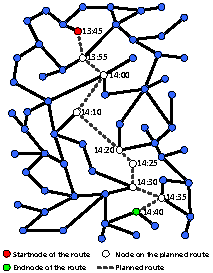
\includegraphics[width=0.43\textwidth, angle=0]{extending/figures/WithinDayReplanning/network_original_route}}%
  {\label{fig:labelNetworkPlannedRoute}}%
  {\qquad}%
  \createsubfigure%
  {Network with exceptional event}%
  {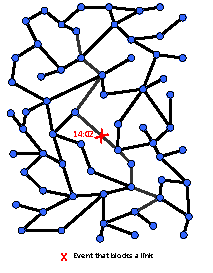
\includegraphics[width=0.43\textwidth, angle=0]{extending/figures/WithinDayReplanning/network_exceptional_event}}%
  {\label{fig:labelNetworkExceptionalEvent}}%
  {\vspace{5mm}}%

  \createsubfigure%
  {Network with exceptional event and planned route}%
  {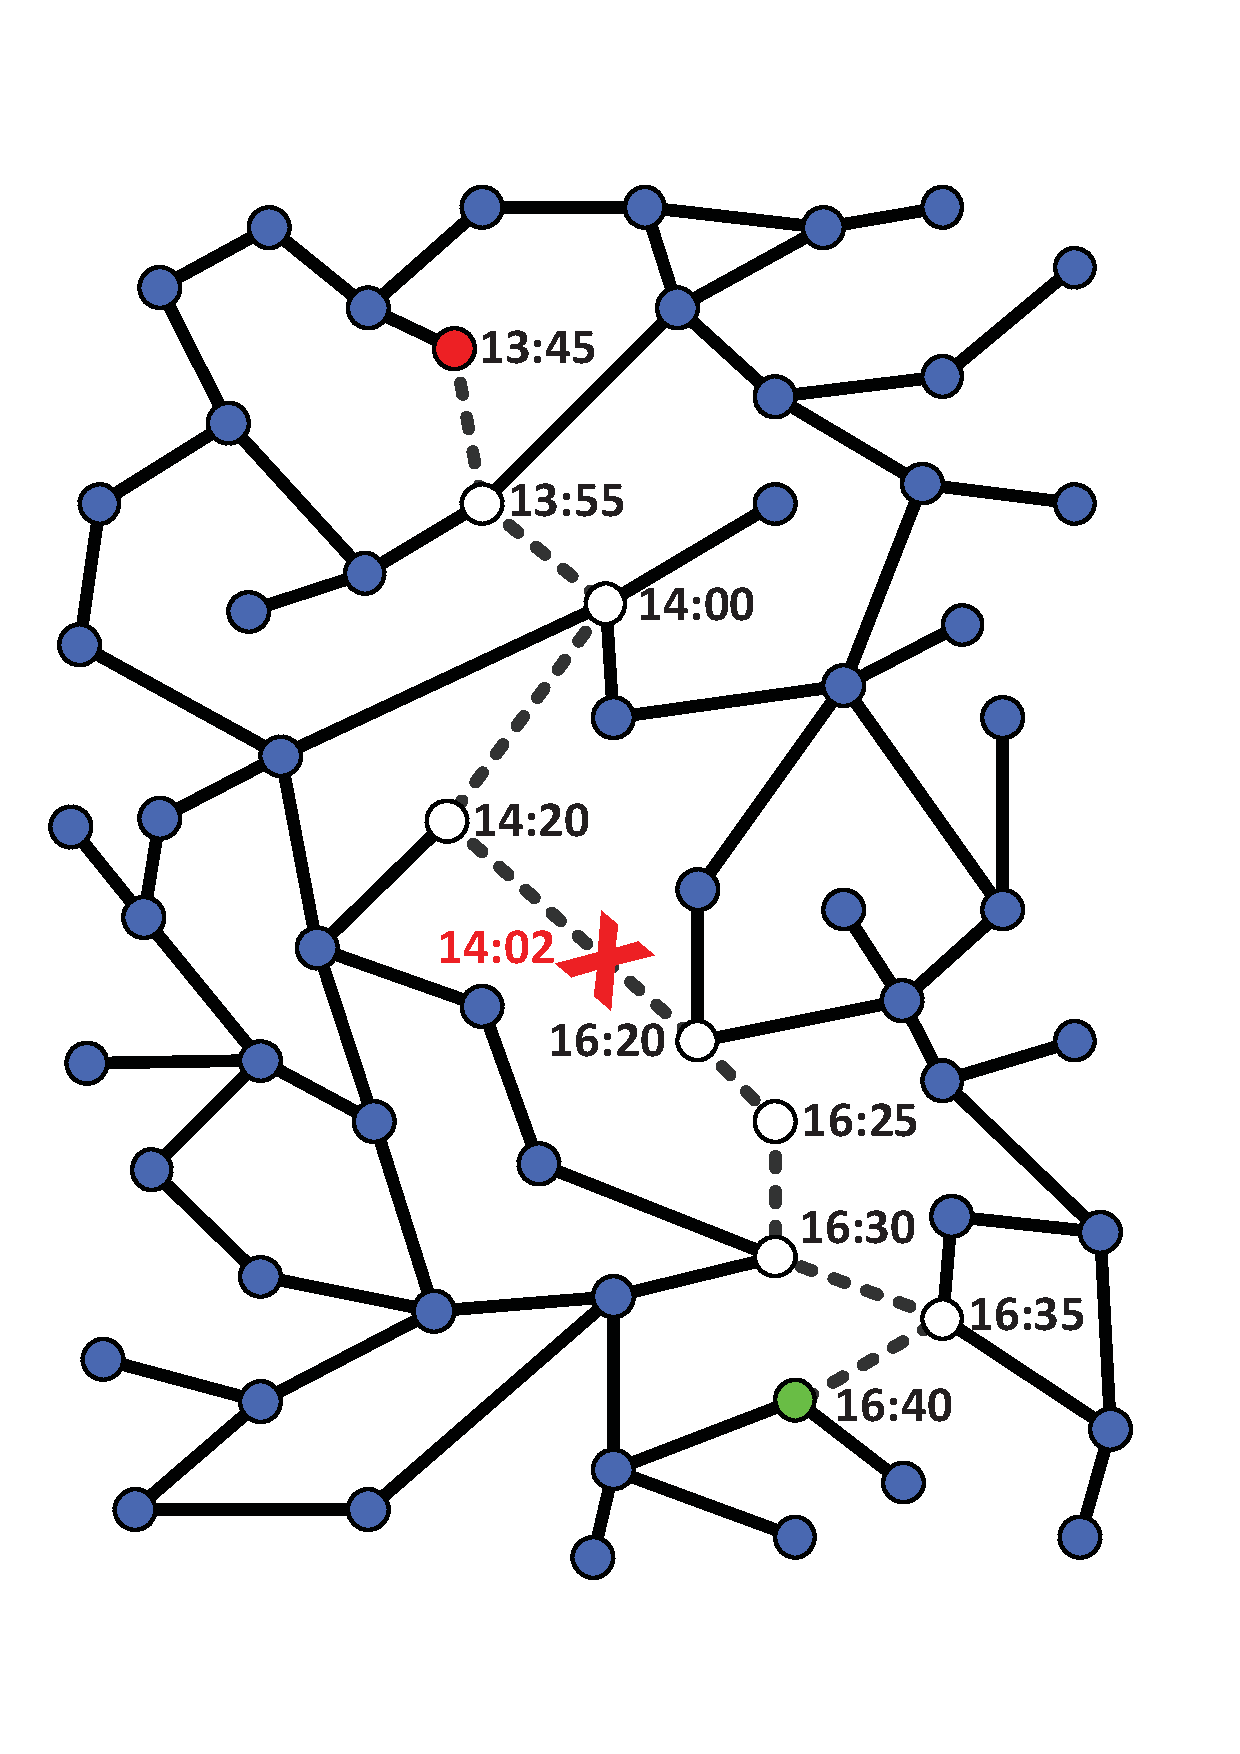
\includegraphics[width=0.43\textwidth, angle=0]{extending/figures/WithinDayReplanning/network_original_route_with_event}}%
  {\label{fig:labelNetworkExceptionalEventPlannedRoute}}%
  {\qquad}%
  \createsubfigure%
  {Network with exceptional event and adapted route}%
  {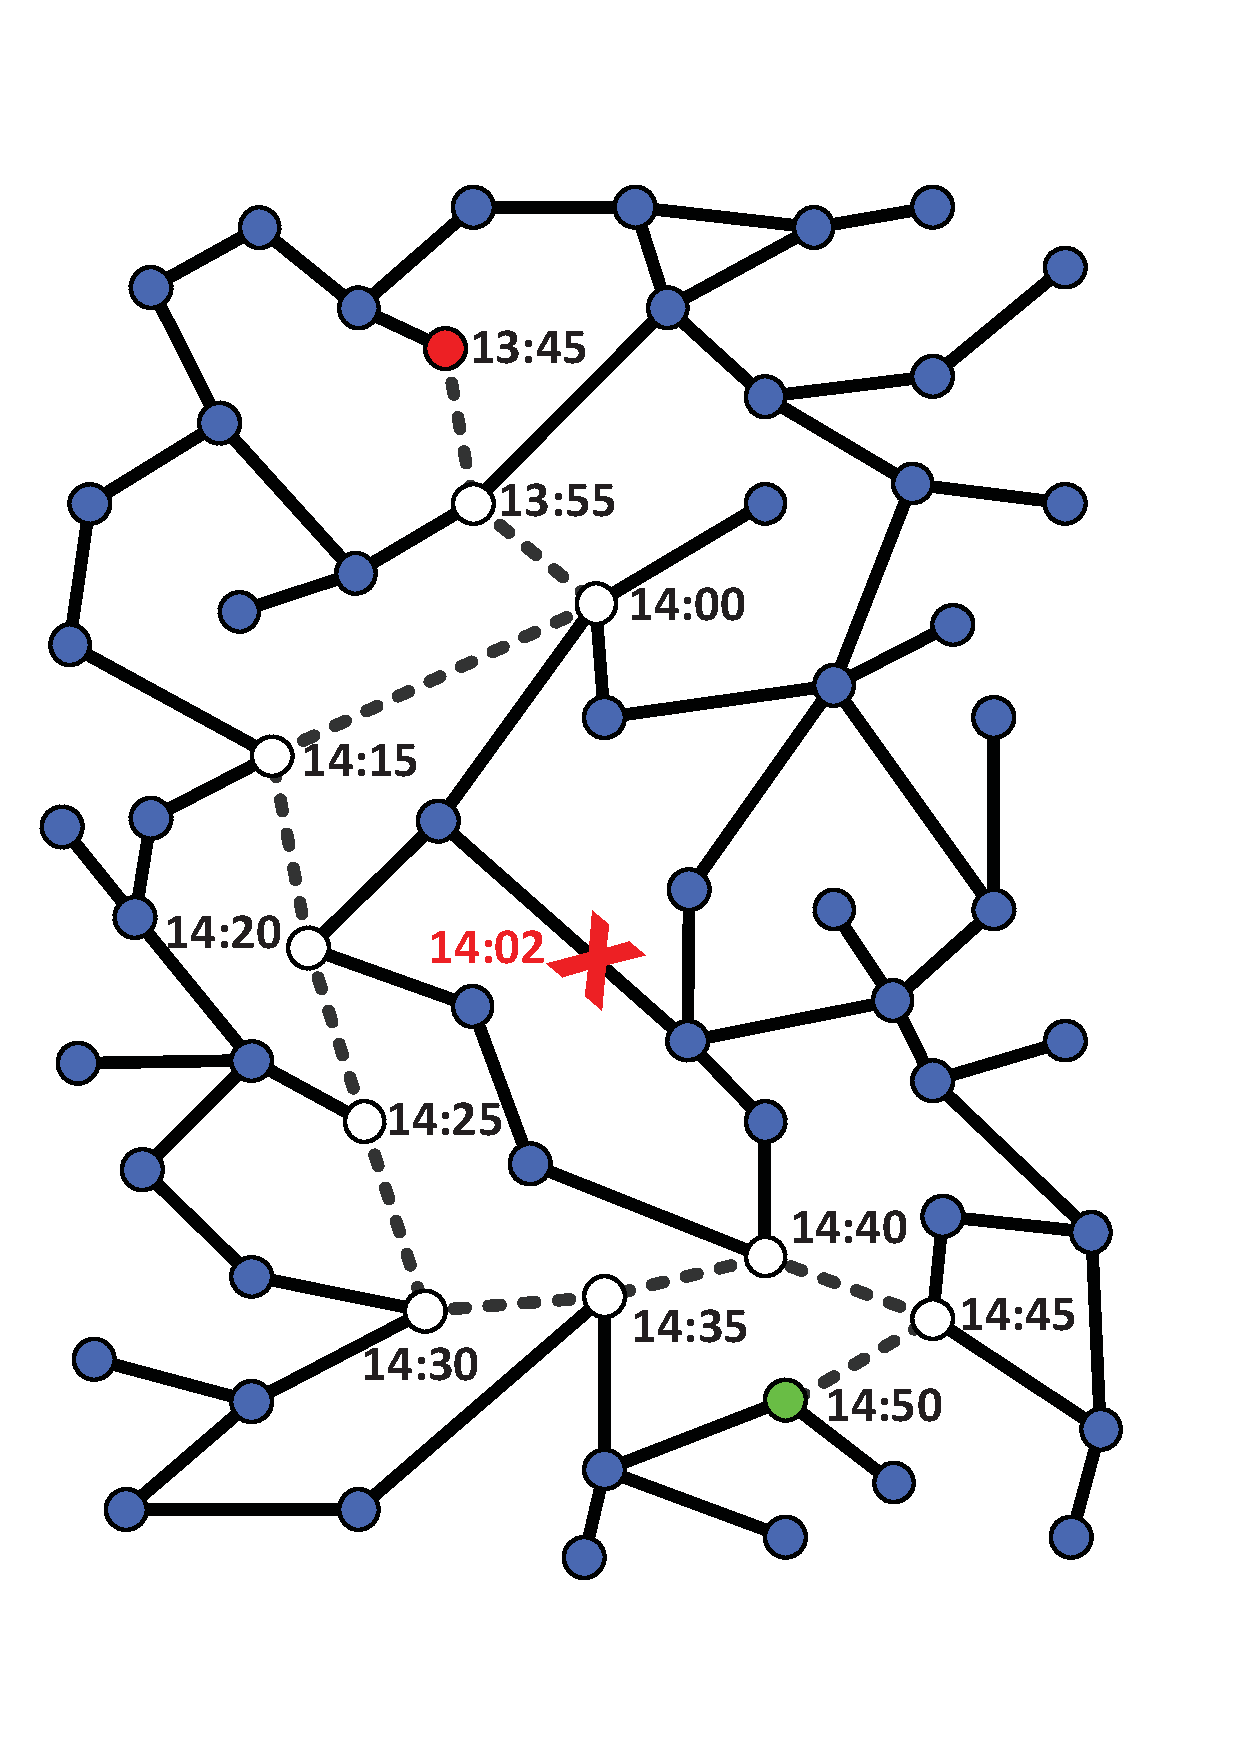
\includegraphics[width=0.43\textwidth, angle=0]{extending/figures/WithinDayReplanning/network_adapted_route_with_event}}%
  {\label{fig:labelNetworkExceptionalEventAdaptedRoute}}%
  {}%
}%
{}
%---------------------------------------------------------------------

Figure \ref{fig:labelExceptionalEventExample} shows a simple example scenario where an iterative approach would produce illogical and faulty results. In Figure \ref{fig:labelNetworkPlannedRoute} an agent's planned route in a sample network is shown, including the times when the driver passes each node of the route. Clearly, those times are only valid if no exceptional event occurs. Figure \ref{fig:labelNetworkExceptionalEvent} shows a link where an event, like an accident, blocks that link for two hours. As a result, the agent reaches its destination two hours later than expected (Figure \ref{fig:labelNetworkExceptionalEventPlannedRoute}). When this scenario is iterated, the agent recognizes that its route has a much higher travel time than expected and therefore it will choose another route. The traffic jam caused by the accident will probably also increase travel times on links next to the blocked link. Therefore, the agent might find a route which is quite different than the original one (Figure \ref{fig:labelNetworkExceptionalEventAdaptedRoute}). A closer look at the node where the new route deviates for the first time from the original one shows that this occurs even before the accident happened, which is unfeasible and illogical.

An obvious solution to avoiding such problems is using an alternative simulation approach without an iterative optimization process. The next section discusses such an approach and the requirements that must be fulfilled.

%%%%%%%%%%%%%%%%%%%%%%%%%%%%%%%%%%%%%%%%%%%%%%%%%%%%%%%%%%%%%%%%%%%%%%
\subsection{Within-Day Replanning Approach}
%%%%%%%%%%%%%%%%%%%%%%%%%%%%%%%%%%%%%%%%%%%%%%%%%%%%%%%%%%%%%%%%%%%%%%

A within-day replanning approach uses a significantly different strategy from that of an iterative approach. Instead of multiple iterations, only a single one is simulated. Thus, it is now essential that agents can adapt their plans during this iteration without having information from previous iterations available. To do so, they have to continuously collect information and take into account their desires, beliefs and intentions when they decide how to (re)act.

While iterative approaches can use best-response modules, a within-day approach has to use something that might be called a best-guess module. Travel times are an obvious example. In an iterative approach, travel times can be collected from the previous iteration or even be averaged over several past iterations. The nearer a stable system is to a relaxed state, the smaller the differences in travel times between two iterations. This is not possible in a within-day approach. Even if an agent has perfect knowledge, it can only assume how the traffic flows will evolve in the future. To do so, it can take different information into account to estimate travel times. It could, for example, take travel times from a typical day without exceptional events and combine them with information it gathers during the simulated day. Depending on the amount and the quality of this information, the agent might rely more or less on its experience.

Therefore, the decision-making process of an agent becomes an important topic. In an iterative approach, each agent has total information and can thus select the best route. Due to limited available information, this is not possible in a within-day approach. One agent could, for example, choose a route where expected travel time is very short, but also very uncertain. Another agent might not be willing to take that risk and therefore select a longer route where the assumed travel time is more reliable. Perception of information might also vary between agents; one could rely on media traffic information, another might ignore it.

Each within-day replanning action is categorized by two parameters---the replanned element of the plan (an activity or a trip) and the point in time when the replanned plan element is executed (right now or at a future point in time). If an activity is replanned, several changes are possible. Its start and end time can be adapted, its location can be changed, it can be dropped, or created new from scratch. For a trip, origin and destination, route, mode of transport and departure time can be replanned. Often replanning one single plan element results in a chain reaction that forces replanning of other plan elements. If, for example, an activity is dropped, the trips from and to this activity have to be merged.

The second parameter categorizing a replanning action depends on when the replanned plan element is executed. This could be either the currently performed plan element or one being performed in the future. Clearly, in a currently performed plan element, not all previously mentioned replanning actions could be conducted. E.g.\ start time of an activity or transport mode of a trip currently being performed can no longer be adapted.

Due to the limited available information, a within-day replanning approach will, in contrast to an iterative approach, not converge to a user equilibrium. Decisions made during the simulated time period may seem to be optimal when they are made. However, evaluated retrospectively, an agent might realize that they were not.

%%%%%%%%%%%%%%%%%%%%%%%%%%%%%%%%%%%%%%%%%%%%%%%%%%%%%%%%%%%%%%%%%%%%%%
\subsection{Combined Approaches} \label{sec:CombinedApproaches}
%%%%%%%%%%%%%%%%%%%%%%%%%%%%%%%%%%%%%%%%%%%%%%%%%%%%%%%%%%%%%%%%%%%%%%

An alternative to iterative or within-day replanning only approaches, is to combine them. An obvious application is solving situations that cannot be planned exactly in advance, like parking or car sharing. An agent is, for example, able to plan a parking activity, but it cannot anticipate which parking spots will be available when the agent arrives. Thus, within-day replanning can be used when the agent starts its parking choice.

Other agents might want to share their cars, so an actual meeting must be confirmed. This can be ensured using within-day replanning. If the driver arrives too early, a \emph{waiting} activity is added to its plan; otherwise the agent being picked up will perform a \emph{waiting} activity until the car arrives.


%%%%%%%%%%%%%%%%%%%%%%%%%%%%%%%%%%%%%%%%%%%%%%%%%%%%%%%%%%%%%%%%%%%%%%
\section{Implementation}
%%%%%%%%%%%%%%%%%%%%%%%%%%%%%%%%%%%%%%%%%%%%%%%%%%%%%%%%%%%%%%%%%%%%%%
\textbf{TODO: describe why there are two different implementations!}


%%%%%%%%%%%%%%%%%%%%%%%%%%%%%%%%%%%%%%%%%%%%%%%%%%%%%%%%%%%%%%%%%%%%%%
\subsection{Plan-based Implementation}
%%%%%%%%%%%%%%%%%%%%%%%%%%%%%%%%%%%%%%%%%%%%%%%%%%%%%%%%%%%%%%%%%%%%%%

When adding within-day replanning to MATSim, its iterative loop (see Figure \ref{fig:matsimcycle}) has to be adapted as shown in Figure \ref{fig:labelWithinDayMATSimLoop}. On one hand, the additional \emph{within-day replanning} module is added, which interacts with the mobility simulation. On the other hand, multiple iterations are only necessary if a combined simulation approach is used.

%---------------------------------------------------------------------
\createfigure%
{(Iterative) within-day replanning MATSim loop}%
{(Iterative) within-day replanning MATSim loop}%
{\label{fig:labelWithinDayMATSimLoop}}%
{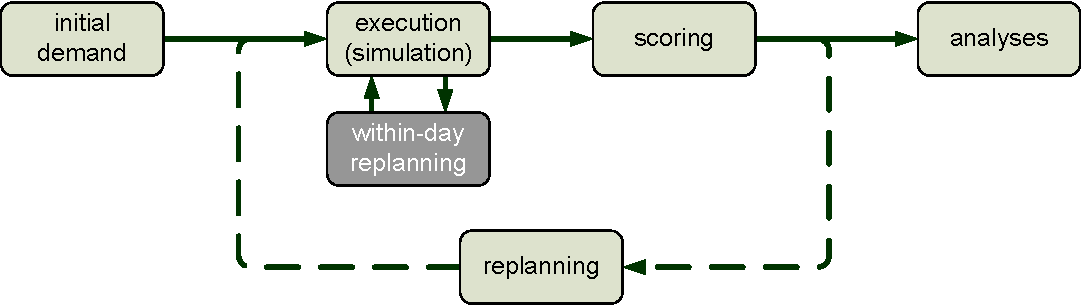
\includegraphics[width=12.5cm, angle=0]{extending/figures/WithinDayReplanning/WithinDayMATSimLoop}}%
{}%
%---------------------------------------------------------------------
\textbf{TODO: redraw this figure using the new (blue) matsim loop?}

The implementation is realized as so-called \emph{MobsimEngine} which can be plugged into the \emph{QSim}. In every simulated time step, the \emph{QSim} iterates over all registered \emph{MobsimEngines} and allows them to simulated the current time step. Besides simulation of the traffic flows, those engines are also able to let agents start or end activities. The engine containing the within-day replanning logic (called \emph{WithinDayEngine}) does not simulate traffic flows but tracks agents and adapts their plans. Doing so is separated into two steps. First, agents whose plans have to be adapted in the current time step are identified. In a second step, the adaption of their plans is performed. 

Figure \ref{fig:labelWithinDayEngine} shows the structure of the \emph{WithinDayEngine}. Multiple \emph{Replanners} can be registered to the engine. Each \emph{Replanner} represents a unique replanning strategy like re-routing or time mutation and uses a set of \emph{Identifiers} which communicate with agents and select those agents who are given the opportunity to adapt their plans. An \emph{Identifier} can be seen as an information-distributing unit, like a radio station or a policeman. Therefore, not every \emph{Identifier} communicates with all agents. For example, agents at home will probably listen to the radio, but agents walking in the park will not. Each \emph{Identifier} returns a list of agents to its superior \emph{Replanner}, which then adapts those agents' plans.

%---------------------------------------------------------------------
\createfigure%
{WithinDayEngine}%
{WithinDayEngine}%
{\label{fig:labelWithinDayEngine}}%
{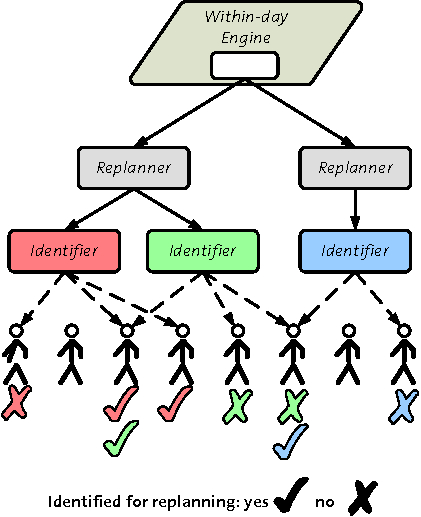
\includegraphics[width=8.0cm, angle=0]{extending/figures/WithinDayReplanning/ReplanningManager}}%
{}
%---------------------------------------------------------------------

There is a division of responsibilties between \emph{Replanners} and \emph{Identifiers}. The first ones are responsible for adapting the agents' plans but they should not check whether an agent should be replanned or not. If, for example, a \emph{Replanner} updates an agent's route, it has to be ensured by the \emph{Identifiers} that only agents who are currently performing a leg are replanned. In turn, \emph{Identifiers} should select agents who have to be replanned but should not change their plans. As a result of this division, the often time consuming replanning of the agents' plans can be performed using parallel threads which leads to an almost linear speed-up. In general, simulation results do not depend on the order in which agents are replanned. \emph{Replanners} which use random numbers are a special case. They have to ensure that their \emph{randon number generator} is re-initialized for every replanned agent using a deterministic value (e.g.~a combination of the agent's Id and the current time step).

Running the \emph{Identifier(s)} to select those agents who have to adapt their plans is performed sequentially. On one hand, an \emph{Identifier's} runtime is typically very short and therefore no significant performance losses are expected. On the other hand, it is a robust design which cannot produce race conditions which could occur if multiple instances of an \emph{Identifier} run concurrently. An example would be an \emph{Identifier} which selects agents on household level, i.e.~if a member of a household is identified, also all other members are added to the list of agents who have to be replanned. In an approach with parallel running instances of an \emph{Identifier}, an instance could identify member A of  a household while concurrently another instance could identify member B of the same household. As a result, the household's members would be twice in the list of agents to be replanned---once added by each \emph{Identifier} instance.

\emph{Replanner} implementations are available for every possible basic change of an agent's scheduled daily plan. Any trips and activities can be adapted, although some replanning operations are not available when trip or activity has already been started. Possible adaptations are:
\begin{compactitem}
    \item current trip (route, destination)
    \item future trip (add, remove, mode, route, origin, destination)
    \item current activity (end time)
    \item future activity (add, remove, location, type, start and end time)
\end{compactitem}

For complex plan adaptations, those basic \emph{Replanners} can be combined. If, for example, an agent currently performing a trip changes the destination of its next activity, routes of the current and next trip have to be adapted.

Additionally, four basic \emph{Identifiers} have been implemented so far. They identify agents, which are...
\begin{compactitem}
    \item performing an activity.
    \item performing an activity which will end in the current time step.
    \item performing a trip.
    \item performing a trip and are going to move to another link.
\end{compactitem}

Often, identifiers have to handle only a subset of the population, e.g.~only male agents or agents which are currently performing a car trip. In order to prevent that the same functionality has to be implemented multiple times, so-called \textit{AgentFilters} are introduced. Their task is to remove agents which do not meet the filter criteria from a set of agents. Using \textit{AgentFilters} not only avoids duplicated code but can also reduce the computation effort. An example would be two \textit{Identifiers} which should identify only agents currently travelling in a certain part of the network. Without \textit{AgentFilters}, each of them would have to track all travelling agents and their current positions. When this functionality is moved to an \textit{AgentFilter}, the two \textit{Identifiers} can share a single instance of that filter.

Basically, simple and re-usable functionality should be implemented as \textit{AgentFilters} while more complex and/or decision making functionality should be part of an \textit{Identifier}. Again, this can be depicted with an example, e.g.\ a scenario in which the search for a parking space is modelled. A filter can be utilized to take only agents into account which are currently travelling by car. The \textit{Identifier} solves the more complex tasks such as deciding when the agent starts its search or selecting the searching strategy to be applied.

Three basic \emph{AgentFilters} have been implemented so far. They filter agents, which are not...
\begin{compactitem}
    \item part of a predefined set of agents.
    \item currently using a transport mode included in a given set.
    \item currently located on a link included in a predefined set.
\end{compactitem}

Besides the logic that identifies agents and adapts their plans, another important part of the within-day replanning framework is code that continuously collects information and provides it to the \emph{Identifiers} which decide based on that data whether agents are replanned or not. In a time step based approach---as it is realized by the \emph{QSim}---collecting, analyzing and aggregating data as well as providing it can be easily realized. Figure~\ref{fig:labelQSimTimeStep} shows the structure of a \emph{QSim's} time step. Each time step is separated into three phases---\emph{before time step}, \emph{do sim step} and \emph{after time step}. During the \emph{do sim step} phase, all registered \emph{MobsimEngines} simulate the current time step. The \emph{before time step} and \emph{after time step} phases allow to execute code before respectively after the simulation of the current time step. A class can collect data like link travel times during the \emph{do sim step} phase. Afterwards, the collected data can be analyzed and aggregated in the \emph{after time step} phase. In the next time step, the \emph{WithinDayEngine's Identifiers} can use that data for their decisions. The \emph{WithinDayEngine} is always the first \emph{MobsimEngine} which executes its \emph{doSimStep} method. This ensures that no agent has changed its state since the \emph{after time step} phase of the previous time step. As a result, the \emph{Identifiers} make their decisions on actual data.

%---------------------------------------------------------------------
\createfigure%
{QSim time step}%
{QSim time step}%
{\label{fig:labelQSimTimeStep}}%
{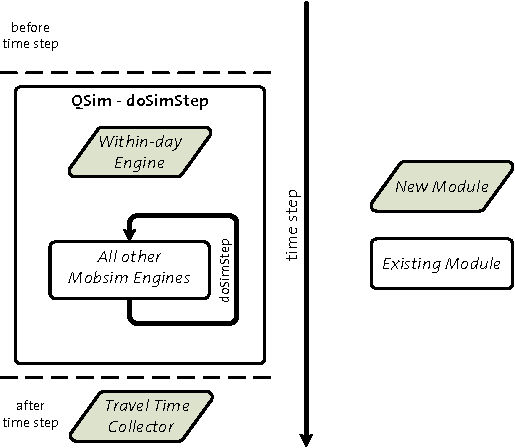
\includegraphics[width=8.0cm, angle=0]{extending/figures/WithinDayReplanning/QSimTimeStep}}%
{}
%---------------------------------------------------------------------

An example for such a class is the so-called \emph{TravelTimeCollector}. Its task is to provide actual link travel times to the \emph{Replanners} by collecting and averaging travel times of agents that have recently passed a link during a given time span. A typical time span is 15~minutes; older link travel times are ignored. Duration of the specific time span has an important impact on travel times reported to the \emph{Replanners}. On one hand, significant changes in link travel times will be communicated very slowly, if the time span is too long. On the other hand, a too short duration will overrate outliers.

The \emph{TravelTimeCollector} is a simple, but efficient implementation of a within-day travel time calculator. It does not implement features like traffic flow predictions or dynamic weighting of recent travel times based on historical data. Due to the abandonment of such features, it is very robust, even in scenarios where traffic flow conditions change dramatically.

%---------------------------------------------------------------------
\createfigure%
{TravelTimeCollector}%
{TravelTimeCollector}%
{\label{fig:labelTravelTimeCollector}}%
{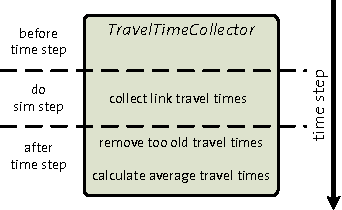
\includegraphics[width=8.0cm, angle=0]{extending/figures/WithinDayReplanning/TravelTimeCollector}}%
{}
%---------------------------------------------------------------------

An important aspect that has to be considered when within-day replanning is used is whether the persons' or only the agents' plans are replanned. In this context, a person is a global object which exists during an entire simulation run. An agent represents a person in the micro-simulation part of an iteration. Moreover, a person has several plans in its memory, an agent only a single one. By default, an agent's plan is only a copy of the plan of the person which is represented. Only the score of the person's plan is updated by MATSim's scoring module. 

In a first one, within-day replanning is used to simulate agents' parking search. A person's plan contains the location where a free parking space is expected. However, if the agent realizes in the micro-simulation that there is no free space left, it starts looking for a free parking spot. As a result, the agent's route is extended. This extension has to be local in the agent's route since it is only necessary in the current iteration
but maybe not in another one where the initially selected parking spot is available.

Creating agents' initial routes using within-day replanning would be an example for an application where persons' plans have to be adapted. By default, creation of those routes is a step performed on person level before the micro-simulation is started for the first time. When this task is moved into the micro-simulation and is performed during their runtime, the created routes have to be still stored in the person's plan. Otherwise they would not be available for later iterations.

The capabilities of this within-day replanning implementation are shown and discussed by \citet{Dobler_PhDThesis_2013} based on two sets of conducted experiments. The first set is based on a model of Zurich city. There it is assumed that the capacities of several arterial roads in the city center are drastically reduced during the morning peak. Travelling agents are given the opportunity to bypass the resulting traffic jams by adapting their routes using within-day replanning. The second set of experiments uses within-day replanning to create agents' initial routes. The results are compared to runs where those routes are created before the simulation is started and without having traffic flow information available.